\documentclass[11pt,a4paper]{article}

\usepackage[utf8]{inputenc}
\usepackage{polski}
\usepackage{graphicx}
\usepackage{graphics}
\usepackage{subfig}
\usepackage{float}
\usepackage{geometry}
\usepackage{amsmath}
\usepackage{color}
\usepackage{enumerate}
\usepackage{indentfirst}
\usepackage{hyperref}
\usepackage{multirow}
\usepackage{array}
\usepackage{url}
\usepackage{longtable} 
\newgeometry{lmargin=2.5cm,rmargin=2.5cm}

\title{}
\author{}
\date{}

\begin{document}
\begin{table}[]
\hspace{-2em}
\begin{tabular}{|c|l|c|c|c|c|}
\hline
	\begin{tabular}[c]{@{}c@{}}Wydział\\ FiIS\end{tabular}&
	\multicolumn{2}{l|}{\begin{tabular}[c]{@{}l@{}}Imię i nazwisko\\ 1. Piotr Kowalczyk\\ 2. Marcin Polok\end{tabular}}&
	\begin{tabular}[c]{@{}c@{}}Rok\\ IV\end{tabular}&
	\begin{tabular}[c]{@{}c@{}}Grupa \\ 2\end{tabular}&
	\begin{tabular}[c]{@{}c@{}}Zespół \\ 2\end{tabular}
\\ \hline
	\begin{tabular}[c]{@{}c@{}}LABORATORIUM\\ DETEKCJI\\ PROMIENIOWANIA\end{tabular}&
	\multicolumn{5}{l|}{\textbf{\begin{tabular}[c]{@{}l@{}}Temat\\ Badanie licznika półprzewodnikowego \end{tabular}}}
\\ \hline
	\begin{tabular}[c]{@{}c@{}}Data wykonania\\ 3.11.2016\end{tabular}&
	\multicolumn{1}{c|}{\begin{tabular}[c]{@{}c@{}}Data oddania\\ 30.11.2016 \end{tabular}}&
	\multicolumn{1}{c|}{\begin{tabular}[c]{@{}c@{}}Zwrot do popr.\\~ \end{tabular}}&
	\multicolumn{1}{c|}{\begin{tabular}[c]{@{}c@{}}Data oddania\\~ \end{tabular}}&
	\multicolumn{1}{c|}{\begin{tabular}[c]{@{}c@{}}Data zaliczenia\\~ \end{tabular}}&
	\multicolumn{1}{c|}{\begin{tabular}[c]{@{}c@{}}OCENA\\~ \end{tabular}}
\\ \hline
\end{tabular}
\end{table}


%%%%%%%%%%%%%%%%%%%%%%%%%%%%%%%%%%%%%%%%%%%%%%%%%%%%%%%%%%%%%%%%%%%%%%%%%%%%%%%%%%%%%%%%%%%%%%%%%%%%%%%%%%%%%%%%%%%%%%%%%%%%%%
%                                                CEL ĆWICZENIA                                                               %
%%%%%%%%%%%%%%%%%%%%%%%%%%%%%%%%%%%%%%%%%%%%%%%%%%%%%%%%%%%%%%%%%%%%%%%%%%%%%%%%%%%%%%%%%%%%%%%%%%%%%%%%%%%%%%%%%%%%%%%%%%%%%%
\section{Wstęp teoretyczny}
pruda piotr
%%%%%%%%%%%%%%%%%%%%%%%%%%%%%%%%%%%%%%%%%%%%%%%%%%%%%%%%%%%%%%%%%%%%%%%%%%%%%%%%%%%%%%%%%%%%%%%%%%%%%%%%%%%%%%%%%%%%%%%%%%%%%%
%                                                PRZEBIEG ĆWICZENIA                                                          %
%%%%%%%%%%%%%%%%%%%%%%%%%%%%%%%%%%%%%%%%%%%%%%%%%%%%%%%%%%%%%%%%%%%%%%%%%%%%%%%%%%%%%%%%%%%%%%%%%%%%%%%%%%%%%%%%%%%%%%%%%%%%%%
\section{Przebieg ćwiczenia}
\begin{itemize}
\item Sprawdzamy poprawność podłączenia układu pomiarowego.
\item Wykonujemy pomiar widma $^{55}Fe$ dla rosnących wartości napięcia polarywacji.
\item Zamiast detektora, pod układ pomiarowy podpinamy generator sygnałów.
\item Ustawiamy generator tak, aby generował sygnał testowy, czyli prostokątny o częstotliwości $100Hz$.
\item Mierzymy odpowiedź analizatora, przy ustalonym czasie pomiaru, na sygnały testowe dla różnych amplitud generowanego sygnału.
\item Odłączamy generator sygnałów.
\item Ponownie mierzymy widmo $^{55}Fe$, dla $U_{bias} = 200V$ oraz $t=300s$.
\item Do pomierzonego widma fitujemy funkcję gaussa, i zapisujemy wyniki.
\item Analogicznie mierzymy i dopasowywujemy widmo dla $^{109}Cd$, dla $U_{bias} = 200V$ oraz $t=300s$.
\item Pomierzyliśmy analogiczne i dopasowaliśmy gaussa dla widma srebra, ale przez niedopatrzenie, zapisaliśmy tylko wyniki fitu.
\end{itemize}

%%%%%%%%%%%%%%%%%%%%%%%%%%%%%%%%%%%%%%%%%%%%%%%%%%%%%%%%%%%%%%%%%%%%%%%%%%%%%%%%%%%%%%%%%%%%%%%%%%%%%%%%%%%%%%%%%%%%%%%%%%%%%%
%                                                WYNIKI                                                                      %
%%%%%%%%%%%%%%%%%%%%%%%%%%%%%%%%%%%%%%%%%%%%%%%%%%%%%%%%%%%%%%%%%%%%%%%%%%%%%%%%%%%%%%%%%%%%%%%%%%%%%%%%%%%%%%%%%%%%%%%%%%%%%%
\section{Wyniki}
\subsection{Pomiar ze źródłem Fe-55.}

\begin{figure}[H]
\centering
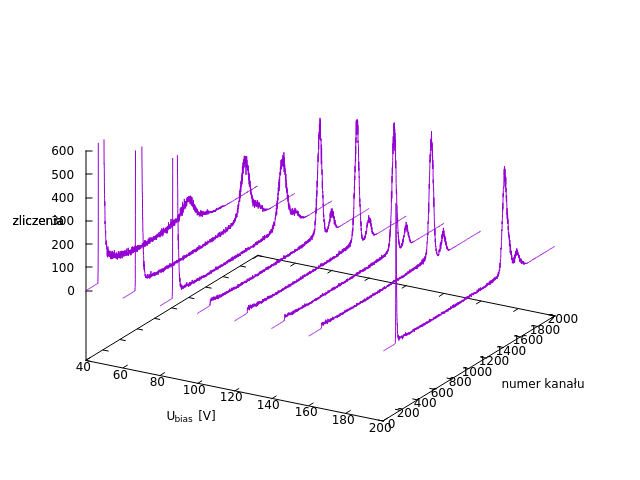
\includegraphics[width=.9\linewidth]{fe.png}
\caption{Widmo żelaza dla napięć polaryzacji 40V, 60V, 80V, 100V, 120V, 140V, 160V, 200V.}
\label{fig1}
\end{figure}

\begin{figure}[H]
\centering
\resizebox{.8\linewidth}{!}{% GNUPLOT: LaTeX picture with Postscript
\begingroup
  \makeatletter
  \providecommand\color[2][]{%
    \GenericError{(gnuplot) \space\space\space\@spaces}{%
      Package color not loaded in conjunction with
      terminal option `colourtext'%
    }{See the gnuplot documentation for explanation.%
    }{Either use 'blacktext' in gnuplot or load the package
      color.sty in LaTeX.}%
    \renewcommand\color[2][]{}%
  }%
  \providecommand\includegraphics[2][]{%
    \GenericError{(gnuplot) \space\space\space\@spaces}{%
      Package graphicx or graphics not loaded%
    }{See the gnuplot documentation for explanation.%
    }{The gnuplot epslatex terminal needs graphicx.sty or graphics.sty.}%
    \renewcommand\includegraphics[2][]{}%
  }%
  \providecommand\rotatebox[2]{#2}%
  \@ifundefined{ifGPcolor}{%
    \newif\ifGPcolor
    \GPcolortrue
  }{}%
  \@ifundefined{ifGPblacktext}{%
    \newif\ifGPblacktext
    \GPblacktexttrue
  }{}%
  % define a \g@addto@macro without @ in the name:
  \let\gplgaddtomacro\g@addto@macro
  % define empty templates for all commands taking text:
  \gdef\gplbacktext{}%
  \gdef\gplfronttext{}%
  \makeatother
  \ifGPblacktext
    % no textcolor at all
    \def\colorrgb#1{}%
    \def\colorgray#1{}%
  \else
    % gray or color?
    \ifGPcolor
      \def\colorrgb#1{\color[rgb]{#1}}%
      \def\colorgray#1{\color[gray]{#1}}%
      \expandafter\def\csname LTw\endcsname{\color{white}}%
      \expandafter\def\csname LTb\endcsname{\color{black}}%
      \expandafter\def\csname LTa\endcsname{\color{black}}%
      \expandafter\def\csname LT0\endcsname{\color[rgb]{1,0,0}}%
      \expandafter\def\csname LT1\endcsname{\color[rgb]{0,1,0}}%
      \expandafter\def\csname LT2\endcsname{\color[rgb]{0,0,1}}%
      \expandafter\def\csname LT3\endcsname{\color[rgb]{1,0,1}}%
      \expandafter\def\csname LT4\endcsname{\color[rgb]{0,1,1}}%
      \expandafter\def\csname LT5\endcsname{\color[rgb]{1,1,0}}%
      \expandafter\def\csname LT6\endcsname{\color[rgb]{0,0,0}}%
      \expandafter\def\csname LT7\endcsname{\color[rgb]{1,0.3,0}}%
      \expandafter\def\csname LT8\endcsname{\color[rgb]{0.5,0.5,0.5}}%
    \else
      % gray
      \def\colorrgb#1{\color{black}}%
      \def\colorgray#1{\color[gray]{#1}}%
      \expandafter\def\csname LTw\endcsname{\color{white}}%
      \expandafter\def\csname LTb\endcsname{\color{black}}%
      \expandafter\def\csname LTa\endcsname{\color{black}}%
      \expandafter\def\csname LT0\endcsname{\color{black}}%
      \expandafter\def\csname LT1\endcsname{\color{black}}%
      \expandafter\def\csname LT2\endcsname{\color{black}}%
      \expandafter\def\csname LT3\endcsname{\color{black}}%
      \expandafter\def\csname LT4\endcsname{\color{black}}%
      \expandafter\def\csname LT5\endcsname{\color{black}}%
      \expandafter\def\csname LT6\endcsname{\color{black}}%
      \expandafter\def\csname LT7\endcsname{\color{black}}%
      \expandafter\def\csname LT8\endcsname{\color{black}}%
    \fi
  \fi
  \setlength{\unitlength}{0.0500bp}%
  \begin{picture}(7200.00,5040.00)%
    \gplgaddtomacro\gplbacktext{%
      \csname LTb\endcsname%
      \put(946,704){\makebox(0,0)[r]{\strut{} 0}}%
      \put(946,1213){\makebox(0,0)[r]{\strut{} 50}}%
      \put(946,1722){\makebox(0,0)[r]{\strut{} 100}}%
      \put(946,2231){\makebox(0,0)[r]{\strut{} 150}}%
      \put(946,2740){\makebox(0,0)[r]{\strut{} 200}}%
      \put(946,3248){\makebox(0,0)[r]{\strut{} 250}}%
      \put(946,3757){\makebox(0,0)[r]{\strut{} 300}}%
      \put(946,4266){\makebox(0,0)[r]{\strut{} 350}}%
      \put(946,4775){\makebox(0,0)[r]{\strut{} 400}}%
      \put(1078,484){\makebox(0,0){\strut{} 0}}%
      \put(2509,484){\makebox(0,0){\strut{} 500}}%
      \put(3941,484){\makebox(0,0){\strut{} 1000}}%
      \put(5372,484){\makebox(0,0){\strut{} 1500}}%
      \put(6803,484){\makebox(0,0){\strut{} 2000}}%
      \put(176,2739){\rotatebox{-270}{\makebox(0,0){\strut{}zliczenia}}}%
      \put(3940,154){\makebox(0,0){\strut{}kanał}}%
    }%
    \gplgaddtomacro\gplfronttext{%
    }%
    \gplbacktext
    \put(0,0){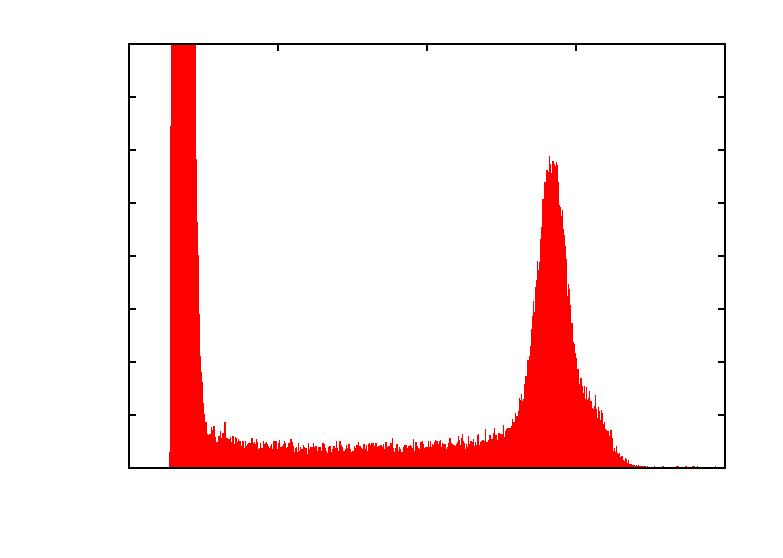
\includegraphics{zelazo_60}}%
    \gplfronttext
  \end{picture}%
\endgroup
}
\caption{Widmo żelaza przy podanym napięciu 60V.}
\label{fig1}
\end{figure}

\begin{figure}[H]
\centering
\resizebox{.8\linewidth}{!}{% GNUPLOT: LaTeX picture with Postscript
\begingroup
  \makeatletter
  \providecommand\color[2][]{%
    \GenericError{(gnuplot) \space\space\space\@spaces}{%
      Package color not loaded in conjunction with
      terminal option `colourtext'%
    }{See the gnuplot documentation for explanation.%
    }{Either use 'blacktext' in gnuplot or load the package
      color.sty in LaTeX.}%
    \renewcommand\color[2][]{}%
  }%
  \providecommand\includegraphics[2][]{%
    \GenericError{(gnuplot) \space\space\space\@spaces}{%
      Package graphicx or graphics not loaded%
    }{See the gnuplot documentation for explanation.%
    }{The gnuplot epslatex terminal needs graphicx.sty or graphics.sty.}%
    \renewcommand\includegraphics[2][]{}%
  }%
  \providecommand\rotatebox[2]{#2}%
  \@ifundefined{ifGPcolor}{%
    \newif\ifGPcolor
    \GPcolortrue
  }{}%
  \@ifundefined{ifGPblacktext}{%
    \newif\ifGPblacktext
    \GPblacktexttrue
  }{}%
  % define a \g@addto@macro without @ in the name:
  \let\gplgaddtomacro\g@addto@macro
  % define empty templates for all commands taking text:
  \gdef\gplbacktext{}%
  \gdef\gplfronttext{}%
  \makeatother
  \ifGPblacktext
    % no textcolor at all
    \def\colorrgb#1{}%
    \def\colorgray#1{}%
  \else
    % gray or color?
    \ifGPcolor
      \def\colorrgb#1{\color[rgb]{#1}}%
      \def\colorgray#1{\color[gray]{#1}}%
      \expandafter\def\csname LTw\endcsname{\color{white}}%
      \expandafter\def\csname LTb\endcsname{\color{black}}%
      \expandafter\def\csname LTa\endcsname{\color{black}}%
      \expandafter\def\csname LT0\endcsname{\color[rgb]{1,0,0}}%
      \expandafter\def\csname LT1\endcsname{\color[rgb]{0,1,0}}%
      \expandafter\def\csname LT2\endcsname{\color[rgb]{0,0,1}}%
      \expandafter\def\csname LT3\endcsname{\color[rgb]{1,0,1}}%
      \expandafter\def\csname LT4\endcsname{\color[rgb]{0,1,1}}%
      \expandafter\def\csname LT5\endcsname{\color[rgb]{1,1,0}}%
      \expandafter\def\csname LT6\endcsname{\color[rgb]{0,0,0}}%
      \expandafter\def\csname LT7\endcsname{\color[rgb]{1,0.3,0}}%
      \expandafter\def\csname LT8\endcsname{\color[rgb]{0.5,0.5,0.5}}%
    \else
      % gray
      \def\colorrgb#1{\color{black}}%
      \def\colorgray#1{\color[gray]{#1}}%
      \expandafter\def\csname LTw\endcsname{\color{white}}%
      \expandafter\def\csname LTb\endcsname{\color{black}}%
      \expandafter\def\csname LTa\endcsname{\color{black}}%
      \expandafter\def\csname LT0\endcsname{\color{black}}%
      \expandafter\def\csname LT1\endcsname{\color{black}}%
      \expandafter\def\csname LT2\endcsname{\color{black}}%
      \expandafter\def\csname LT3\endcsname{\color{black}}%
      \expandafter\def\csname LT4\endcsname{\color{black}}%
      \expandafter\def\csname LT5\endcsname{\color{black}}%
      \expandafter\def\csname LT6\endcsname{\color{black}}%
      \expandafter\def\csname LT7\endcsname{\color{black}}%
      \expandafter\def\csname LT8\endcsname{\color{black}}%
    \fi
  \fi
  \setlength{\unitlength}{0.0500bp}%
  \begin{picture}(7200.00,5040.00)%
    \gplgaddtomacro\gplbacktext{%
      \csname LTb\endcsname%
      \put(946,704){\makebox(0,0)[r]{\strut{} 0}}%
      \put(946,1213){\makebox(0,0)[r]{\strut{} 50}}%
      \put(946,1722){\makebox(0,0)[r]{\strut{} 100}}%
      \put(946,2231){\makebox(0,0)[r]{\strut{} 150}}%
      \put(946,2740){\makebox(0,0)[r]{\strut{} 200}}%
      \put(946,3248){\makebox(0,0)[r]{\strut{} 250}}%
      \put(946,3757){\makebox(0,0)[r]{\strut{} 300}}%
      \put(946,4266){\makebox(0,0)[r]{\strut{} 350}}%
      \put(946,4775){\makebox(0,0)[r]{\strut{} 400}}%
      \put(1078,484){\makebox(0,0){\strut{} 0}}%
      \put(2509,484){\makebox(0,0){\strut{} 500}}%
      \put(3941,484){\makebox(0,0){\strut{} 1000}}%
      \put(5372,484){\makebox(0,0){\strut{} 1500}}%
      \put(6803,484){\makebox(0,0){\strut{} 2000}}%
      \put(176,2739){\rotatebox{-270}{\makebox(0,0){\strut{}zliczenia}}}%
      \put(3940,154){\makebox(0,0){\strut{}kanał}}%
    }%
    \gplgaddtomacro\gplfronttext{%
    }%
    \gplbacktext
    \put(0,0){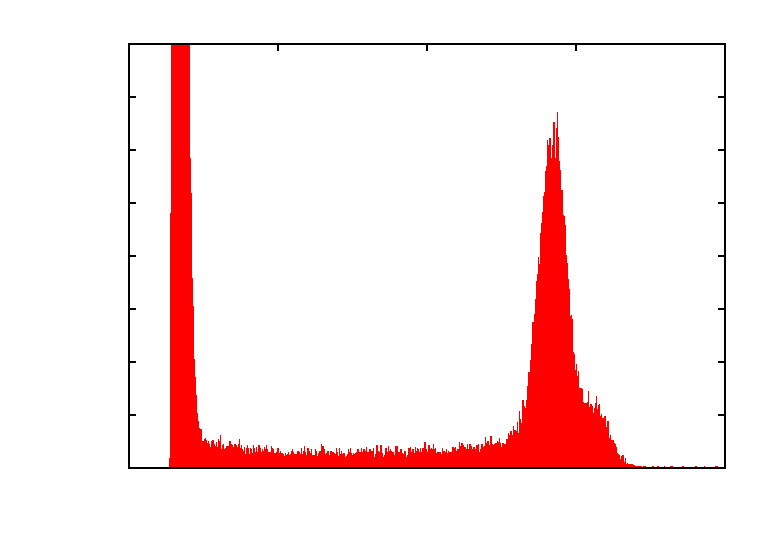
\includegraphics{zelazo_80}}%
    \gplfronttext
  \end{picture}%
\endgroup
}
\caption{Widmo żelaza przy podanym napięciu 80V.}
\label{fig1}
\end{figure}

\begin{figure}[H]
\centering
\resizebox{.8\linewidth}{!}{% GNUPLOT: LaTeX picture with Postscript
\begingroup
  \makeatletter
  \providecommand\color[2][]{%
    \GenericError{(gnuplot) \space\space\space\@spaces}{%
      Package color not loaded in conjunction with
      terminal option `colourtext'%
    }{See the gnuplot documentation for explanation.%
    }{Either use 'blacktext' in gnuplot or load the package
      color.sty in LaTeX.}%
    \renewcommand\color[2][]{}%
  }%
  \providecommand\includegraphics[2][]{%
    \GenericError{(gnuplot) \space\space\space\@spaces}{%
      Package graphicx or graphics not loaded%
    }{See the gnuplot documentation for explanation.%
    }{The gnuplot epslatex terminal needs graphicx.sty or graphics.sty.}%
    \renewcommand\includegraphics[2][]{}%
  }%
  \providecommand\rotatebox[2]{#2}%
  \@ifundefined{ifGPcolor}{%
    \newif\ifGPcolor
    \GPcolortrue
  }{}%
  \@ifundefined{ifGPblacktext}{%
    \newif\ifGPblacktext
    \GPblacktexttrue
  }{}%
  % define a \g@addto@macro without @ in the name:
  \let\gplgaddtomacro\g@addto@macro
  % define empty templates for all commands taking text:
  \gdef\gplbacktext{}%
  \gdef\gplfronttext{}%
  \makeatother
  \ifGPblacktext
    % no textcolor at all
    \def\colorrgb#1{}%
    \def\colorgray#1{}%
  \else
    % gray or color?
    \ifGPcolor
      \def\colorrgb#1{\color[rgb]{#1}}%
      \def\colorgray#1{\color[gray]{#1}}%
      \expandafter\def\csname LTw\endcsname{\color{white}}%
      \expandafter\def\csname LTb\endcsname{\color{black}}%
      \expandafter\def\csname LTa\endcsname{\color{black}}%
      \expandafter\def\csname LT0\endcsname{\color[rgb]{1,0,0}}%
      \expandafter\def\csname LT1\endcsname{\color[rgb]{0,1,0}}%
      \expandafter\def\csname LT2\endcsname{\color[rgb]{0,0,1}}%
      \expandafter\def\csname LT3\endcsname{\color[rgb]{1,0,1}}%
      \expandafter\def\csname LT4\endcsname{\color[rgb]{0,1,1}}%
      \expandafter\def\csname LT5\endcsname{\color[rgb]{1,1,0}}%
      \expandafter\def\csname LT6\endcsname{\color[rgb]{0,0,0}}%
      \expandafter\def\csname LT7\endcsname{\color[rgb]{1,0.3,0}}%
      \expandafter\def\csname LT8\endcsname{\color[rgb]{0.5,0.5,0.5}}%
    \else
      % gray
      \def\colorrgb#1{\color{black}}%
      \def\colorgray#1{\color[gray]{#1}}%
      \expandafter\def\csname LTw\endcsname{\color{white}}%
      \expandafter\def\csname LTb\endcsname{\color{black}}%
      \expandafter\def\csname LTa\endcsname{\color{black}}%
      \expandafter\def\csname LT0\endcsname{\color{black}}%
      \expandafter\def\csname LT1\endcsname{\color{black}}%
      \expandafter\def\csname LT2\endcsname{\color{black}}%
      \expandafter\def\csname LT3\endcsname{\color{black}}%
      \expandafter\def\csname LT4\endcsname{\color{black}}%
      \expandafter\def\csname LT5\endcsname{\color{black}}%
      \expandafter\def\csname LT6\endcsname{\color{black}}%
      \expandafter\def\csname LT7\endcsname{\color{black}}%
      \expandafter\def\csname LT8\endcsname{\color{black}}%
    \fi
  \fi
  \setlength{\unitlength}{0.0500bp}%
  \begin{picture}(7200.00,5040.00)%
    \gplgaddtomacro\gplbacktext{%
      \csname LTb\endcsname%
      \put(946,704){\makebox(0,0)[r]{\strut{} 0}}%
      \put(946,1383){\makebox(0,0)[r]{\strut{} 100}}%
      \put(946,2061){\makebox(0,0)[r]{\strut{} 200}}%
      \put(946,2740){\makebox(0,0)[r]{\strut{} 300}}%
      \put(946,3418){\makebox(0,0)[r]{\strut{} 400}}%
      \put(946,4097){\makebox(0,0)[r]{\strut{} 500}}%
      \put(946,4775){\makebox(0,0)[r]{\strut{} 600}}%
      \put(1078,484){\makebox(0,0){\strut{} 0}}%
      \put(2509,484){\makebox(0,0){\strut{} 500}}%
      \put(3941,484){\makebox(0,0){\strut{} 1000}}%
      \put(5372,484){\makebox(0,0){\strut{} 1500}}%
      \put(6803,484){\makebox(0,0){\strut{} 2000}}%
      \put(176,2739){\rotatebox{-270}{\makebox(0,0){\strut{}zliczenia}}}%
      \put(3940,154){\makebox(0,0){\strut{}kanał}}%
    }%
    \gplgaddtomacro\gplfronttext{%
    }%
    \gplbacktext
    \put(0,0){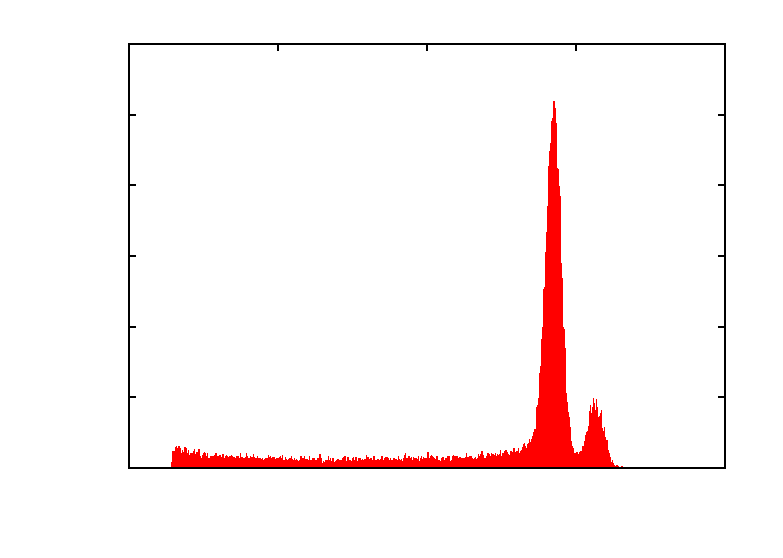
\includegraphics{zelazo_100}}%
    \gplfronttext
  \end{picture}%
\endgroup
}
\caption{Widmo żelaza przy podanym napięciu 100V.}
\label{fig1}
\end{figure}

\begin{figure}[H]
\centering
\resizebox{.8\linewidth}{!}{% GNUPLOT: LaTeX picture with Postscript
\begingroup
  \makeatletter
  \providecommand\color[2][]{%
    \GenericError{(gnuplot) \space\space\space\@spaces}{%
      Package color not loaded in conjunction with
      terminal option `colourtext'%
    }{See the gnuplot documentation for explanation.%
    }{Either use 'blacktext' in gnuplot or load the package
      color.sty in LaTeX.}%
    \renewcommand\color[2][]{}%
  }%
  \providecommand\includegraphics[2][]{%
    \GenericError{(gnuplot) \space\space\space\@spaces}{%
      Package graphicx or graphics not loaded%
    }{See the gnuplot documentation for explanation.%
    }{The gnuplot epslatex terminal needs graphicx.sty or graphics.sty.}%
    \renewcommand\includegraphics[2][]{}%
  }%
  \providecommand\rotatebox[2]{#2}%
  \@ifundefined{ifGPcolor}{%
    \newif\ifGPcolor
    \GPcolortrue
  }{}%
  \@ifundefined{ifGPblacktext}{%
    \newif\ifGPblacktext
    \GPblacktexttrue
  }{}%
  % define a \g@addto@macro without @ in the name:
  \let\gplgaddtomacro\g@addto@macro
  % define empty templates for all commands taking text:
  \gdef\gplbacktext{}%
  \gdef\gplfronttext{}%
  \makeatother
  \ifGPblacktext
    % no textcolor at all
    \def\colorrgb#1{}%
    \def\colorgray#1{}%
  \else
    % gray or color?
    \ifGPcolor
      \def\colorrgb#1{\color[rgb]{#1}}%
      \def\colorgray#1{\color[gray]{#1}}%
      \expandafter\def\csname LTw\endcsname{\color{white}}%
      \expandafter\def\csname LTb\endcsname{\color{black}}%
      \expandafter\def\csname LTa\endcsname{\color{black}}%
      \expandafter\def\csname LT0\endcsname{\color[rgb]{1,0,0}}%
      \expandafter\def\csname LT1\endcsname{\color[rgb]{0,1,0}}%
      \expandafter\def\csname LT2\endcsname{\color[rgb]{0,0,1}}%
      \expandafter\def\csname LT3\endcsname{\color[rgb]{1,0,1}}%
      \expandafter\def\csname LT4\endcsname{\color[rgb]{0,1,1}}%
      \expandafter\def\csname LT5\endcsname{\color[rgb]{1,1,0}}%
      \expandafter\def\csname LT6\endcsname{\color[rgb]{0,0,0}}%
      \expandafter\def\csname LT7\endcsname{\color[rgb]{1,0.3,0}}%
      \expandafter\def\csname LT8\endcsname{\color[rgb]{0.5,0.5,0.5}}%
    \else
      % gray
      \def\colorrgb#1{\color{black}}%
      \def\colorgray#1{\color[gray]{#1}}%
      \expandafter\def\csname LTw\endcsname{\color{white}}%
      \expandafter\def\csname LTb\endcsname{\color{black}}%
      \expandafter\def\csname LTa\endcsname{\color{black}}%
      \expandafter\def\csname LT0\endcsname{\color{black}}%
      \expandafter\def\csname LT1\endcsname{\color{black}}%
      \expandafter\def\csname LT2\endcsname{\color{black}}%
      \expandafter\def\csname LT3\endcsname{\color{black}}%
      \expandafter\def\csname LT4\endcsname{\color{black}}%
      \expandafter\def\csname LT5\endcsname{\color{black}}%
      \expandafter\def\csname LT6\endcsname{\color{black}}%
      \expandafter\def\csname LT7\endcsname{\color{black}}%
      \expandafter\def\csname LT8\endcsname{\color{black}}%
    \fi
  \fi
  \setlength{\unitlength}{0.0500bp}%
  \begin{picture}(7200.00,5040.00)%
    \gplgaddtomacro\gplbacktext{%
      \csname LTb\endcsname%
      \put(946,704){\makebox(0,0)[r]{\strut{} 0}}%
      \put(946,1383){\makebox(0,0)[r]{\strut{} 100}}%
      \put(946,2061){\makebox(0,0)[r]{\strut{} 200}}%
      \put(946,2740){\makebox(0,0)[r]{\strut{} 300}}%
      \put(946,3418){\makebox(0,0)[r]{\strut{} 400}}%
      \put(946,4097){\makebox(0,0)[r]{\strut{} 500}}%
      \put(946,4775){\makebox(0,0)[r]{\strut{} 600}}%
      \put(1078,484){\makebox(0,0){\strut{} 0}}%
      \put(2509,484){\makebox(0,0){\strut{} 500}}%
      \put(3941,484){\makebox(0,0){\strut{} 1000}}%
      \put(5372,484){\makebox(0,0){\strut{} 1500}}%
      \put(6803,484){\makebox(0,0){\strut{} 2000}}%
      \put(176,2739){\rotatebox{-270}{\makebox(0,0){\strut{}zliczenia}}}%
      \put(3940,154){\makebox(0,0){\strut{}kanał}}%
    }%
    \gplgaddtomacro\gplfronttext{%
    }%
    \gplbacktext
    \put(0,0){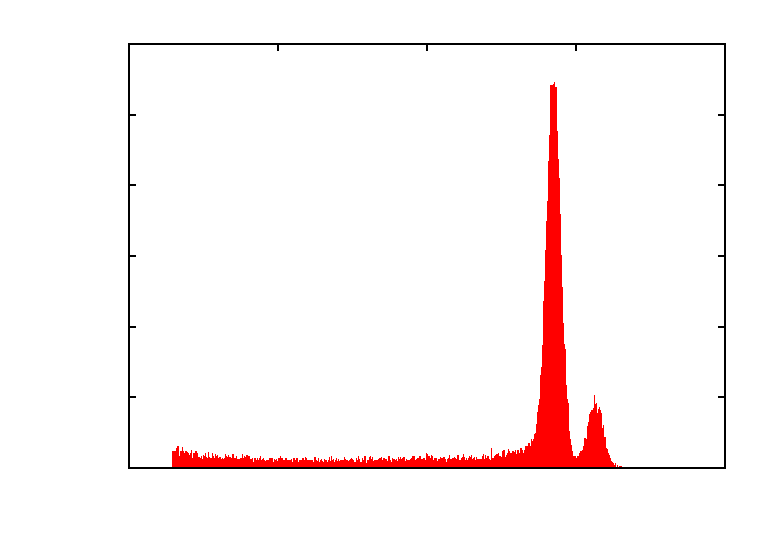
\includegraphics{zelazo_120}}%
    \gplfronttext
  \end{picture}%
\endgroup
}
\caption{Widmo żelaza przy podanym napięciu 120V.}
\label{fig1}
\end{figure}

\begin{figure}[H]
\centering
\resizebox{.8\linewidth}{!}{% GNUPLOT: LaTeX picture with Postscript
\begingroup
  \makeatletter
  \providecommand\color[2][]{%
    \GenericError{(gnuplot) \space\space\space\@spaces}{%
      Package color not loaded in conjunction with
      terminal option `colourtext'%
    }{See the gnuplot documentation for explanation.%
    }{Either use 'blacktext' in gnuplot or load the package
      color.sty in LaTeX.}%
    \renewcommand\color[2][]{}%
  }%
  \providecommand\includegraphics[2][]{%
    \GenericError{(gnuplot) \space\space\space\@spaces}{%
      Package graphicx or graphics not loaded%
    }{See the gnuplot documentation for explanation.%
    }{The gnuplot epslatex terminal needs graphicx.sty or graphics.sty.}%
    \renewcommand\includegraphics[2][]{}%
  }%
  \providecommand\rotatebox[2]{#2}%
  \@ifundefined{ifGPcolor}{%
    \newif\ifGPcolor
    \GPcolortrue
  }{}%
  \@ifundefined{ifGPblacktext}{%
    \newif\ifGPblacktext
    \GPblacktexttrue
  }{}%
  % define a \g@addto@macro without @ in the name:
  \let\gplgaddtomacro\g@addto@macro
  % define empty templates for all commands taking text:
  \gdef\gplbacktext{}%
  \gdef\gplfronttext{}%
  \makeatother
  \ifGPblacktext
    % no textcolor at all
    \def\colorrgb#1{}%
    \def\colorgray#1{}%
  \else
    % gray or color?
    \ifGPcolor
      \def\colorrgb#1{\color[rgb]{#1}}%
      \def\colorgray#1{\color[gray]{#1}}%
      \expandafter\def\csname LTw\endcsname{\color{white}}%
      \expandafter\def\csname LTb\endcsname{\color{black}}%
      \expandafter\def\csname LTa\endcsname{\color{black}}%
      \expandafter\def\csname LT0\endcsname{\color[rgb]{1,0,0}}%
      \expandafter\def\csname LT1\endcsname{\color[rgb]{0,1,0}}%
      \expandafter\def\csname LT2\endcsname{\color[rgb]{0,0,1}}%
      \expandafter\def\csname LT3\endcsname{\color[rgb]{1,0,1}}%
      \expandafter\def\csname LT4\endcsname{\color[rgb]{0,1,1}}%
      \expandafter\def\csname LT5\endcsname{\color[rgb]{1,1,0}}%
      \expandafter\def\csname LT6\endcsname{\color[rgb]{0,0,0}}%
      \expandafter\def\csname LT7\endcsname{\color[rgb]{1,0.3,0}}%
      \expandafter\def\csname LT8\endcsname{\color[rgb]{0.5,0.5,0.5}}%
    \else
      % gray
      \def\colorrgb#1{\color{black}}%
      \def\colorgray#1{\color[gray]{#1}}%
      \expandafter\def\csname LTw\endcsname{\color{white}}%
      \expandafter\def\csname LTb\endcsname{\color{black}}%
      \expandafter\def\csname LTa\endcsname{\color{black}}%
      \expandafter\def\csname LT0\endcsname{\color{black}}%
      \expandafter\def\csname LT1\endcsname{\color{black}}%
      \expandafter\def\csname LT2\endcsname{\color{black}}%
      \expandafter\def\csname LT3\endcsname{\color{black}}%
      \expandafter\def\csname LT4\endcsname{\color{black}}%
      \expandafter\def\csname LT5\endcsname{\color{black}}%
      \expandafter\def\csname LT6\endcsname{\color{black}}%
      \expandafter\def\csname LT7\endcsname{\color{black}}%
      \expandafter\def\csname LT8\endcsname{\color{black}}%
    \fi
  \fi
  \setlength{\unitlength}{0.0500bp}%
  \begin{picture}(7200.00,5040.00)%
    \gplgaddtomacro\gplbacktext{%
      \csname LTb\endcsname%
      \put(946,704){\makebox(0,0)[r]{\strut{} 0}}%
      \put(946,1383){\makebox(0,0)[r]{\strut{} 100}}%
      \put(946,2061){\makebox(0,0)[r]{\strut{} 200}}%
      \put(946,2740){\makebox(0,0)[r]{\strut{} 300}}%
      \put(946,3418){\makebox(0,0)[r]{\strut{} 400}}%
      \put(946,4097){\makebox(0,0)[r]{\strut{} 500}}%
      \put(946,4775){\makebox(0,0)[r]{\strut{} 600}}%
      \put(1078,484){\makebox(0,0){\strut{} 0}}%
      \put(2509,484){\makebox(0,0){\strut{} 500}}%
      \put(3941,484){\makebox(0,0){\strut{} 1000}}%
      \put(5372,484){\makebox(0,0){\strut{} 1500}}%
      \put(6803,484){\makebox(0,0){\strut{} 2000}}%
      \put(176,2739){\rotatebox{-270}{\makebox(0,0){\strut{}zliczenia}}}%
      \put(3940,154){\makebox(0,0){\strut{}kanał}}%
    }%
    \gplgaddtomacro\gplfronttext{%
    }%
    \gplbacktext
    \put(0,0){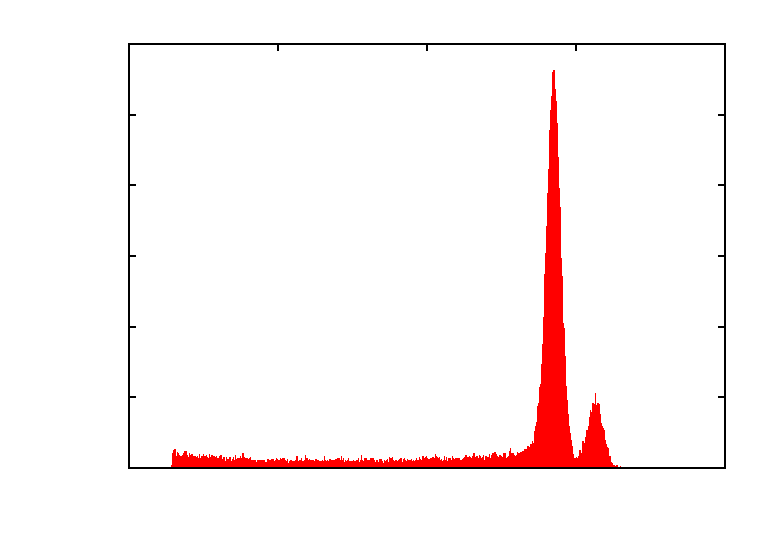
\includegraphics{zelazo_140}}%
    \gplfronttext
  \end{picture}%
\endgroup
}
\caption{Widmo żelaza przy podanym napięciu 140V.}
\label{fig1}
\end{figure}

\begin{figure}[H]
\centering
\resizebox{.8\linewidth}{!}{% GNUPLOT: LaTeX picture with Postscript
\begingroup
  \makeatletter
  \providecommand\color[2][]{%
    \GenericError{(gnuplot) \space\space\space\@spaces}{%
      Package color not loaded in conjunction with
      terminal option `colourtext'%
    }{See the gnuplot documentation for explanation.%
    }{Either use 'blacktext' in gnuplot or load the package
      color.sty in LaTeX.}%
    \renewcommand\color[2][]{}%
  }%
  \providecommand\includegraphics[2][]{%
    \GenericError{(gnuplot) \space\space\space\@spaces}{%
      Package graphicx or graphics not loaded%
    }{See the gnuplot documentation for explanation.%
    }{The gnuplot epslatex terminal needs graphicx.sty or graphics.sty.}%
    \renewcommand\includegraphics[2][]{}%
  }%
  \providecommand\rotatebox[2]{#2}%
  \@ifundefined{ifGPcolor}{%
    \newif\ifGPcolor
    \GPcolortrue
  }{}%
  \@ifundefined{ifGPblacktext}{%
    \newif\ifGPblacktext
    \GPblacktexttrue
  }{}%
  % define a \g@addto@macro without @ in the name:
  \let\gplgaddtomacro\g@addto@macro
  % define empty templates for all commands taking text:
  \gdef\gplbacktext{}%
  \gdef\gplfronttext{}%
  \makeatother
  \ifGPblacktext
    % no textcolor at all
    \def\colorrgb#1{}%
    \def\colorgray#1{}%
  \else
    % gray or color?
    \ifGPcolor
      \def\colorrgb#1{\color[rgb]{#1}}%
      \def\colorgray#1{\color[gray]{#1}}%
      \expandafter\def\csname LTw\endcsname{\color{white}}%
      \expandafter\def\csname LTb\endcsname{\color{black}}%
      \expandafter\def\csname LTa\endcsname{\color{black}}%
      \expandafter\def\csname LT0\endcsname{\color[rgb]{1,0,0}}%
      \expandafter\def\csname LT1\endcsname{\color[rgb]{0,1,0}}%
      \expandafter\def\csname LT2\endcsname{\color[rgb]{0,0,1}}%
      \expandafter\def\csname LT3\endcsname{\color[rgb]{1,0,1}}%
      \expandafter\def\csname LT4\endcsname{\color[rgb]{0,1,1}}%
      \expandafter\def\csname LT5\endcsname{\color[rgb]{1,1,0}}%
      \expandafter\def\csname LT6\endcsname{\color[rgb]{0,0,0}}%
      \expandafter\def\csname LT7\endcsname{\color[rgb]{1,0.3,0}}%
      \expandafter\def\csname LT8\endcsname{\color[rgb]{0.5,0.5,0.5}}%
    \else
      % gray
      \def\colorrgb#1{\color{black}}%
      \def\colorgray#1{\color[gray]{#1}}%
      \expandafter\def\csname LTw\endcsname{\color{white}}%
      \expandafter\def\csname LTb\endcsname{\color{black}}%
      \expandafter\def\csname LTa\endcsname{\color{black}}%
      \expandafter\def\csname LT0\endcsname{\color{black}}%
      \expandafter\def\csname LT1\endcsname{\color{black}}%
      \expandafter\def\csname LT2\endcsname{\color{black}}%
      \expandafter\def\csname LT3\endcsname{\color{black}}%
      \expandafter\def\csname LT4\endcsname{\color{black}}%
      \expandafter\def\csname LT5\endcsname{\color{black}}%
      \expandafter\def\csname LT6\endcsname{\color{black}}%
      \expandafter\def\csname LT7\endcsname{\color{black}}%
      \expandafter\def\csname LT8\endcsname{\color{black}}%
    \fi
  \fi
  \setlength{\unitlength}{0.0500bp}%
  \begin{picture}(7200.00,5040.00)%
    \gplgaddtomacro\gplbacktext{%
      \csname LTb\endcsname%
      \put(946,704){\makebox(0,0)[r]{\strut{} 0}}%
      \put(946,1383){\makebox(0,0)[r]{\strut{} 100}}%
      \put(946,2061){\makebox(0,0)[r]{\strut{} 200}}%
      \put(946,2740){\makebox(0,0)[r]{\strut{} 300}}%
      \put(946,3418){\makebox(0,0)[r]{\strut{} 400}}%
      \put(946,4097){\makebox(0,0)[r]{\strut{} 500}}%
      \put(946,4775){\makebox(0,0)[r]{\strut{} 600}}%
      \put(1078,484){\makebox(0,0){\strut{} 0}}%
      \put(2509,484){\makebox(0,0){\strut{} 500}}%
      \put(3941,484){\makebox(0,0){\strut{} 1000}}%
      \put(5372,484){\makebox(0,0){\strut{} 1500}}%
      \put(6803,484){\makebox(0,0){\strut{} 2000}}%
      \put(176,2739){\rotatebox{-270}{\makebox(0,0){\strut{}zliczenia}}}%
      \put(3940,154){\makebox(0,0){\strut{}kanał}}%
    }%
    \gplgaddtomacro\gplfronttext{%
    }%
    \gplbacktext
    \put(0,0){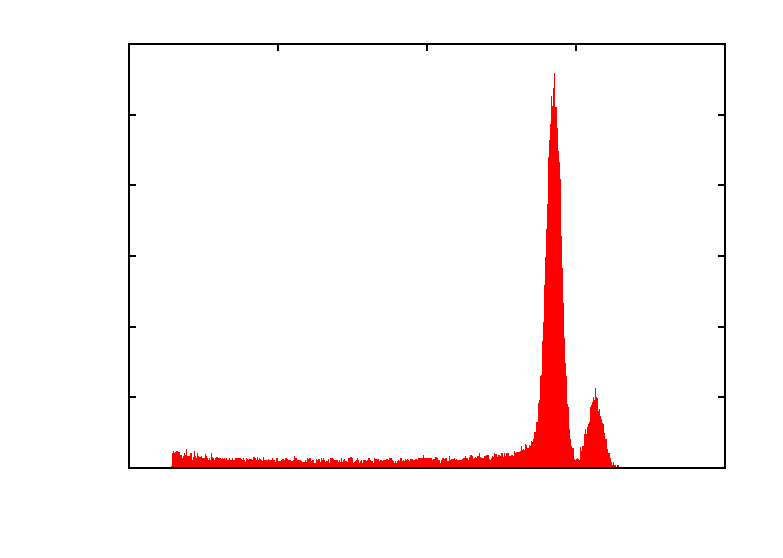
\includegraphics{zelazo_160}}%
    \gplfronttext
  \end{picture}%
\endgroup
}
\caption{Widmo żelaza przy podanym napięciu 160V.}
\label{fig1}
\end{figure}

\begin{figure}[H]
\centering
\resizebox{.8\linewidth}{!}{% GNUPLOT: LaTeX picture with Postscript
\begingroup
  \makeatletter
  \providecommand\color[2][]{%
    \GenericError{(gnuplot) \space\space\space\@spaces}{%
      Package color not loaded in conjunction with
      terminal option `colourtext'%
    }{See the gnuplot documentation for explanation.%
    }{Either use 'blacktext' in gnuplot or load the package
      color.sty in LaTeX.}%
    \renewcommand\color[2][]{}%
  }%
  \providecommand\includegraphics[2][]{%
    \GenericError{(gnuplot) \space\space\space\@spaces}{%
      Package graphicx or graphics not loaded%
    }{See the gnuplot documentation for explanation.%
    }{The gnuplot epslatex terminal needs graphicx.sty or graphics.sty.}%
    \renewcommand\includegraphics[2][]{}%
  }%
  \providecommand\rotatebox[2]{#2}%
  \@ifundefined{ifGPcolor}{%
    \newif\ifGPcolor
    \GPcolortrue
  }{}%
  \@ifundefined{ifGPblacktext}{%
    \newif\ifGPblacktext
    \GPblacktexttrue
  }{}%
  % define a \g@addto@macro without @ in the name:
  \let\gplgaddtomacro\g@addto@macro
  % define empty templates for all commands taking text:
  \gdef\gplbacktext{}%
  \gdef\gplfronttext{}%
  \makeatother
  \ifGPblacktext
    % no textcolor at all
    \def\colorrgb#1{}%
    \def\colorgray#1{}%
  \else
    % gray or color?
    \ifGPcolor
      \def\colorrgb#1{\color[rgb]{#1}}%
      \def\colorgray#1{\color[gray]{#1}}%
      \expandafter\def\csname LTw\endcsname{\color{white}}%
      \expandafter\def\csname LTb\endcsname{\color{black}}%
      \expandafter\def\csname LTa\endcsname{\color{black}}%
      \expandafter\def\csname LT0\endcsname{\color[rgb]{1,0,0}}%
      \expandafter\def\csname LT1\endcsname{\color[rgb]{0,1,0}}%
      \expandafter\def\csname LT2\endcsname{\color[rgb]{0,0,1}}%
      \expandafter\def\csname LT3\endcsname{\color[rgb]{1,0,1}}%
      \expandafter\def\csname LT4\endcsname{\color[rgb]{0,1,1}}%
      \expandafter\def\csname LT5\endcsname{\color[rgb]{1,1,0}}%
      \expandafter\def\csname LT6\endcsname{\color[rgb]{0,0,0}}%
      \expandafter\def\csname LT7\endcsname{\color[rgb]{1,0.3,0}}%
      \expandafter\def\csname LT8\endcsname{\color[rgb]{0.5,0.5,0.5}}%
    \else
      % gray
      \def\colorrgb#1{\color{black}}%
      \def\colorgray#1{\color[gray]{#1}}%
      \expandafter\def\csname LTw\endcsname{\color{white}}%
      \expandafter\def\csname LTb\endcsname{\color{black}}%
      \expandafter\def\csname LTa\endcsname{\color{black}}%
      \expandafter\def\csname LT0\endcsname{\color{black}}%
      \expandafter\def\csname LT1\endcsname{\color{black}}%
      \expandafter\def\csname LT2\endcsname{\color{black}}%
      \expandafter\def\csname LT3\endcsname{\color{black}}%
      \expandafter\def\csname LT4\endcsname{\color{black}}%
      \expandafter\def\csname LT5\endcsname{\color{black}}%
      \expandafter\def\csname LT6\endcsname{\color{black}}%
      \expandafter\def\csname LT7\endcsname{\color{black}}%
      \expandafter\def\csname LT8\endcsname{\color{black}}%
    \fi
  \fi
  \setlength{\unitlength}{0.0500bp}%
  \begin{picture}(7200.00,5040.00)%
    \gplgaddtomacro\gplbacktext{%
      \csname LTb\endcsname%
      \put(946,704){\makebox(0,0)[r]{\strut{} 0}}%
      \put(946,1286){\makebox(0,0)[r]{\strut{} 100}}%
      \put(946,1867){\makebox(0,0)[r]{\strut{} 200}}%
      \put(946,2449){\makebox(0,0)[r]{\strut{} 300}}%
      \put(946,3030){\makebox(0,0)[r]{\strut{} 400}}%
      \put(946,3612){\makebox(0,0)[r]{\strut{} 500}}%
      \put(946,4193){\makebox(0,0)[r]{\strut{} 600}}%
      \put(946,4775){\makebox(0,0)[r]{\strut{} 700}}%
      \put(1078,484){\makebox(0,0){\strut{} 0}}%
      \put(2509,484){\makebox(0,0){\strut{} 500}}%
      \put(3941,484){\makebox(0,0){\strut{} 1000}}%
      \put(5372,484){\makebox(0,0){\strut{} 1500}}%
      \put(6803,484){\makebox(0,0){\strut{} 2000}}%
      \put(176,2739){\rotatebox{-270}{\makebox(0,0){\strut{}zliczenia}}}%
      \put(3940,154){\makebox(0,0){\strut{}kanał}}%
    }%
    \gplgaddtomacro\gplfronttext{%
    }%
    \gplbacktext
    \put(0,0){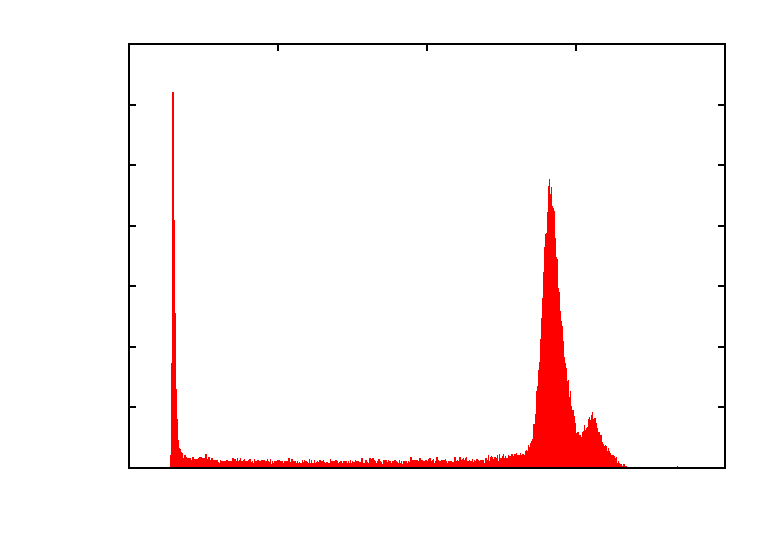
\includegraphics{zelazo_200}}%
    \gplfronttext
  \end{picture}%
\endgroup
}
\caption{Widmo żelaza przy podanym napięciu 200V.}
\label{fig1}
\end{figure}

\subsection{Pomiar z generatorem sygnałów.}
Do danych dopasowano prostą(\ref{fit_gen}) i na tej podstawie obliczono amplitudę odpowiadającą kanałowi 1424. 
Otrzymano $A = 205,7$mV.
Następnie obliczono ładunek zebrany na kondensatorze separującym generator z analizatorem. 
Czynnik $\frac{1}{45}$ wynika z dzielnika napięcia w układzie, natomiast $C_f$ to pojemność tego kondensatora.
$$
Q=\frac{A}{45} \cdot C_f = \frac{0,2057}{45}\cdot 5,75\cdot 10^{-14} [\text{C}] = 2,62\cdot 10^{-16} [\text{C}]
$$
Dzieląc ten ładunek przez ładunek elektronu otrzymujemy ilość par jakie pojawiłyby się w detektorze w tym kanale.
$$
N_0 = Q/e = 1643,04
$$
Ostatecznie biorąc średnią ważoną linii K$_{\alpha 1}$ i K$_{\alpha 2}$ manganu ze źródła żelaza
$$
\text{K}_{\alpha 1\&2} = \frac{5,898*100 + 5,887*50}{150} [\text{keV}]=5,8943 [\text{keV}]
$$
i dzieląc tę wartość przez $N_0$ otrzymujemy pracę wyjścia w detektorze:
\begin{equation}
	W = \frac{\text{K}_{\alpha 1\&2}}{N_0} = 3,587 [\text{eV}].
\end{equation}
Jest to wartość zgodna z oczekiwaną wartością $3,6$eV.

\begin{equation}
	K = 7529(99)[\text{1/V}] \cdot A -125(65)
	\label{fit_gen}
\end{equation}
\begin{figure}[H]
\centering
\resizebox{.8\linewidth}{!}{% GNUPLOT: LaTeX picture with Postscript
\begingroup
  \makeatletter
  \providecommand\color[2][]{%
    \GenericError{(gnuplot) \space\space\space\@spaces}{%
      Package color not loaded in conjunction with
      terminal option `colourtext'%
    }{See the gnuplot documentation for explanation.%
    }{Either use 'blacktext' in gnuplot or load the package
      color.sty in LaTeX.}%
    \renewcommand\color[2][]{}%
  }%
  \providecommand\includegraphics[2][]{%
    \GenericError{(gnuplot) \space\space\space\@spaces}{%
      Package graphicx or graphics not loaded%
    }{See the gnuplot documentation for explanation.%
    }{The gnuplot epslatex terminal needs graphicx.sty or graphics.sty.}%
    \renewcommand\includegraphics[2][]{}%
  }%
  \providecommand\rotatebox[2]{#2}%
  \@ifundefined{ifGPcolor}{%
    \newif\ifGPcolor
    \GPcolortrue
  }{}%
  \@ifundefined{ifGPblacktext}{%
    \newif\ifGPblacktext
    \GPblacktexttrue
  }{}%
  % define a \g@addto@macro without @ in the name:
  \let\gplgaddtomacro\g@addto@macro
  % define empty templates for all commands taking text:
  \gdef\gplbacktext{}%
  \gdef\gplfronttext{}%
  \makeatother
  \ifGPblacktext
    % no textcolor at all
    \def\colorrgb#1{}%
    \def\colorgray#1{}%
  \else
    % gray or color?
    \ifGPcolor
      \def\colorrgb#1{\color[rgb]{#1}}%
      \def\colorgray#1{\color[gray]{#1}}%
      \expandafter\def\csname LTw\endcsname{\color{white}}%
      \expandafter\def\csname LTb\endcsname{\color{black}}%
      \expandafter\def\csname LTa\endcsname{\color{black}}%
      \expandafter\def\csname LT0\endcsname{\color[rgb]{1,0,0}}%
      \expandafter\def\csname LT1\endcsname{\color[rgb]{0,1,0}}%
      \expandafter\def\csname LT2\endcsname{\color[rgb]{0,0,1}}%
      \expandafter\def\csname LT3\endcsname{\color[rgb]{1,0,1}}%
      \expandafter\def\csname LT4\endcsname{\color[rgb]{0,1,1}}%
      \expandafter\def\csname LT5\endcsname{\color[rgb]{1,1,0}}%
      \expandafter\def\csname LT6\endcsname{\color[rgb]{0,0,0}}%
      \expandafter\def\csname LT7\endcsname{\color[rgb]{1,0.3,0}}%
      \expandafter\def\csname LT8\endcsname{\color[rgb]{0.5,0.5,0.5}}%
    \else
      % gray
      \def\colorrgb#1{\color{black}}%
      \def\colorgray#1{\color[gray]{#1}}%
      \expandafter\def\csname LTw\endcsname{\color{white}}%
      \expandafter\def\csname LTb\endcsname{\color{black}}%
      \expandafter\def\csname LTa\endcsname{\color{black}}%
      \expandafter\def\csname LT0\endcsname{\color{black}}%
      \expandafter\def\csname LT1\endcsname{\color{black}}%
      \expandafter\def\csname LT2\endcsname{\color{black}}%
      \expandafter\def\csname LT3\endcsname{\color{black}}%
      \expandafter\def\csname LT4\endcsname{\color{black}}%
      \expandafter\def\csname LT5\endcsname{\color{black}}%
      \expandafter\def\csname LT6\endcsname{\color{black}}%
      \expandafter\def\csname LT7\endcsname{\color{black}}%
      \expandafter\def\csname LT8\endcsname{\color{black}}%
    \fi
  \fi
  \setlength{\unitlength}{0.0500bp}%
  \begin{picture}(7200.00,5040.00)%
    \gplgaddtomacro\gplbacktext{%
      \csname LTb\endcsname%
      \put(1078,704){\makebox(0,0)[r]{\strut{} 0}}%
      \put(1078,1156){\makebox(0,0)[r]{\strut{} 1000}}%
      \put(1078,1609){\makebox(0,0)[r]{\strut{} 2000}}%
      \put(1078,2061){\makebox(0,0)[r]{\strut{} 3000}}%
      \put(1078,2513){\makebox(0,0)[r]{\strut{} 4000}}%
      \put(1078,2966){\makebox(0,0)[r]{\strut{} 5000}}%
      \put(1078,3418){\makebox(0,0)[r]{\strut{} 6000}}%
      \put(1078,3870){\makebox(0,0)[r]{\strut{} 7000}}%
      \put(1078,4323){\makebox(0,0)[r]{\strut{} 8000}}%
      \put(1078,4775){\makebox(0,0)[r]{\strut{} 9000}}%
      \put(1210,484){\makebox(0,0){\strut{} 0}}%
      \put(2227,484){\makebox(0,0){\strut{} 0.2}}%
      \put(3244,484){\makebox(0,0){\strut{} 0.4}}%
      \put(4261,484){\makebox(0,0){\strut{} 0.6}}%
      \put(5278,484){\makebox(0,0){\strut{} 0.8}}%
      \put(6295,484){\makebox(0,0){\strut{} 1}}%
      \put(176,2739){\rotatebox{-270}{\makebox(0,0){\strut{}kanał K}}}%
      \put(4006,154){\makebox(0,0){\strut{}Amplituda sygnału A}}%
    }%
    \gplgaddtomacro\gplfronttext{%
    }%
    \gplbacktext
    \put(0,0){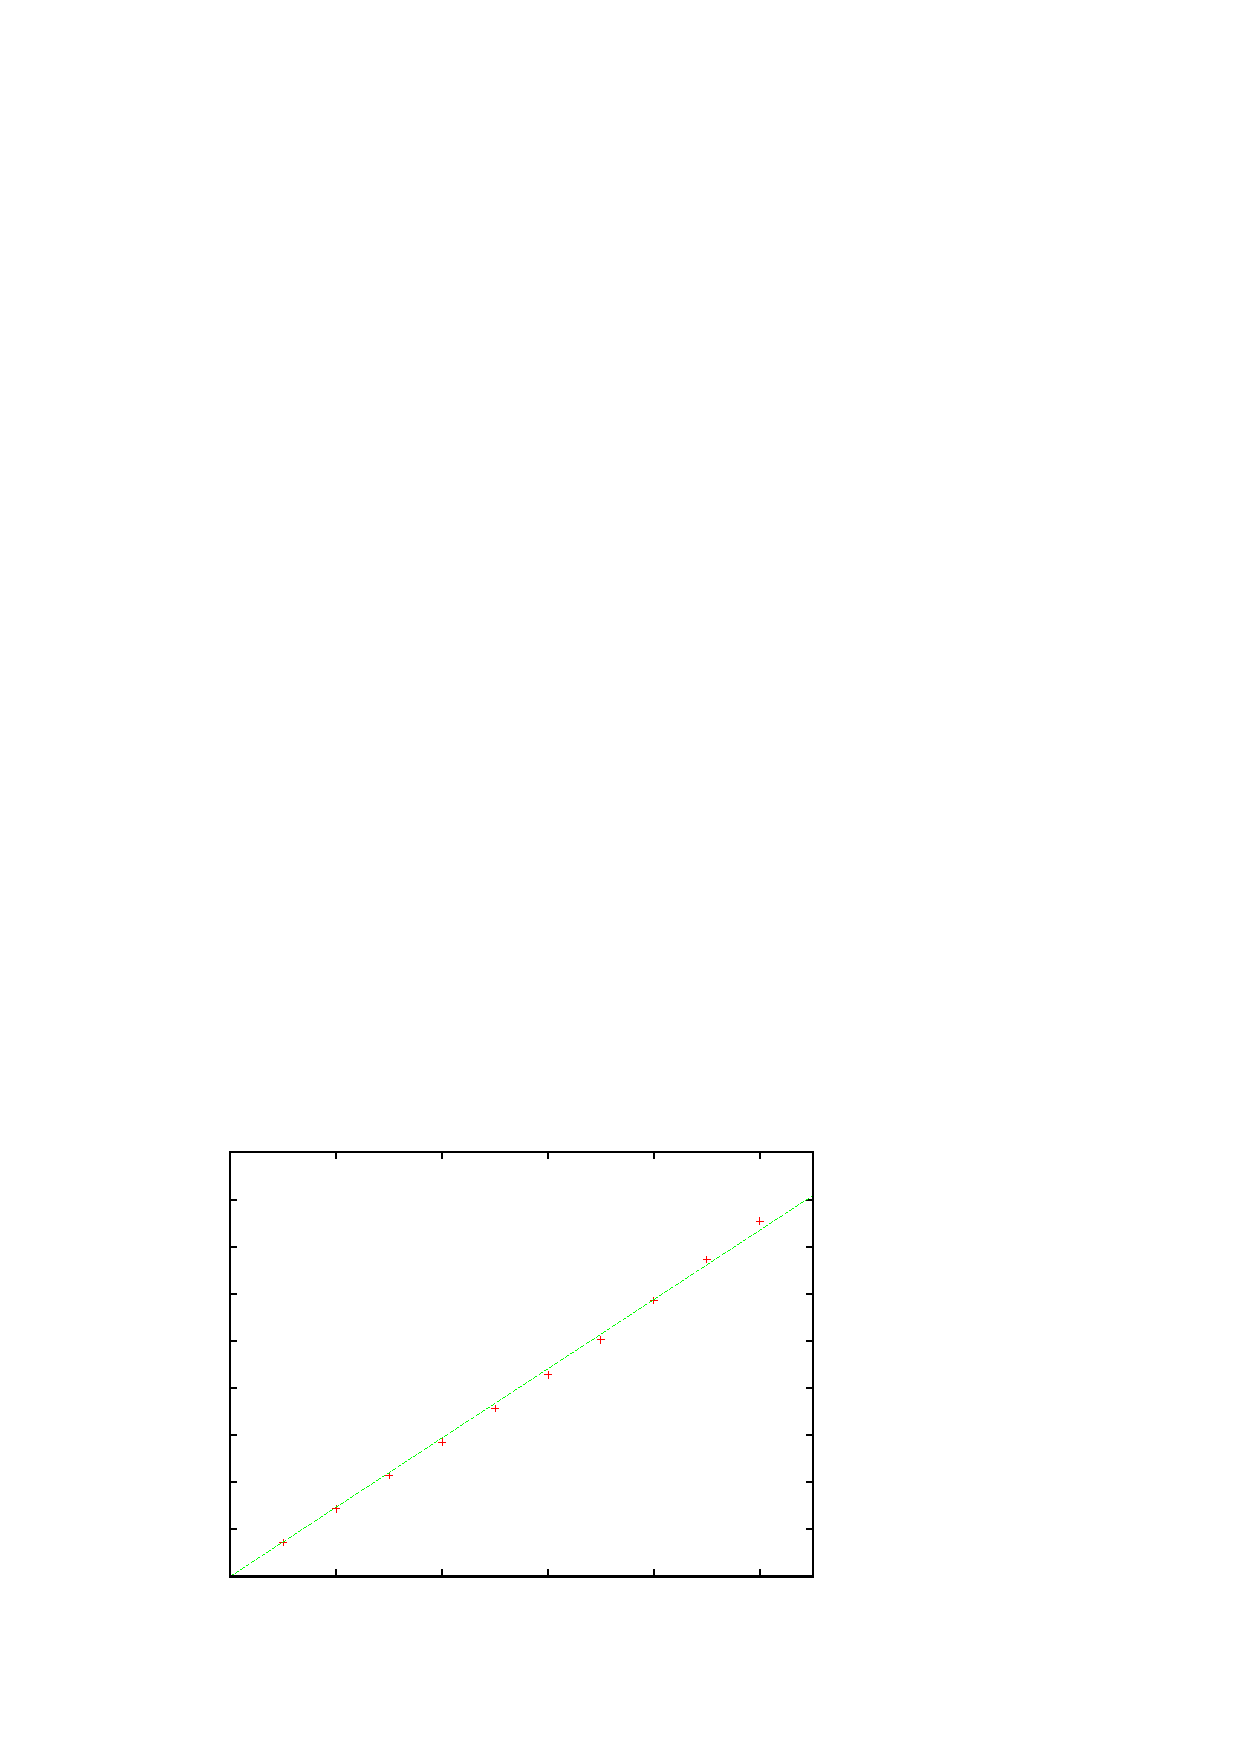
\includegraphics{generator}}%
    \gplfronttext
  \end{picture}%
\endgroup
}
\caption{Pomiar z podłączonym generatorem sygnałów.}
\label{fig1}
\end{figure}

\subsection{Pomiar współczynnika Fano}
\begin{equation}
	\sigma_{całk.}^2 = \sigma_{detektor}^2 + \sigma_{szum}^2
	\label{sigmy}
\end{equation}
\begin{equation}
	\sigma_{detektor}^2 = F\cdot N_0
	\label{fano}
\end{equation}
Przy użyciu generatora sygnałów zmierzono również szerokość połówkową odpowiadającą kanałowi 1424:
$$FWHM_{gen} = 46,92.$$
Założono przy tym, że odpowiada to wariancji szumu w równaniu(\ref{sigmy}), czyli
$$\sigma_{szum} = \frac{46,92}{2,35} = 19,966~ \text{kanału}. $$
Zmierzono również szerokość połówkową żelaza i otrzymano
$$FWHM_{Fe} = 55,34.$$
Założono, że odpowiada to $\sigma_{całk.}$, więc
$$\sigma_{całk.} = \frac{55,34}{2,35} = 23,549~ \text{kanału}.$$
Implikuje to, że $\sigma_{detektor}^2 = 155,91$ kanału.
Korzystając ze wzoru na współczynnik Fano (\ref{fano}) otrzymujemy
$$ F = \frac{\sigma_{detektor}^2}{N_0} = \frac{155,91}{1643,04} = 0,095.$$
Po zaokrągleniu do dzięsiotej częsći po przecinku otrzymujemy dokładnie spodziewaną wartość $0,1$.
\section{Wnioski}

\section{Dane pomiarowe}

\begin{longtable}{c|cc|cc}
	\caption{Pomiary pików i ich szerokości połówkowych. Źródłem było Fe-55.}\\
\label{dt2}
 &\multicolumn{2}{c|}{k$_{\alpha}$}	&\multicolumn{2}{c}{k$_{\beta}$} \\
U[V]	&peak	&FWHM	&peak	&FWHM\\ \hline
\endhead
200	&1425,31	&56,14	&1565,58	&52,93 \\
160	&1425,11	&54,3	&1563,44	&36,29 \\
140	&1424,3		&51,79	&1562,68	&44,91 \\
120	&1424,21	&54,79	&1565,34	&51,33 \\
100	&1423,45	&58,1	&1558,64	&44,7 \\
80	&1423,45	&74,27	&-	&- \\
\end{longtable}

\begin{thebibliography}{9}
\bibitem{skrypt1}
Skrypt Ćwiczenia laboratoryjne z jądrowych metod pomiarowych dostępny pod adresem:\\http://winntbg.bg.agh.edu.pl/skrypty3/0364/dziunikowski-kalita.pdf 
\end{thebibliography}
\end{document}
